\documentclass{article}
\usepackage{tikz}
\usetikzlibrary{arrows.meta}
% 箭头符号
% 在路径的起始或结束位置使用箭头,需要使用arrows.meta库,参考section 16
% 使用箭头的格式: arrows=<start_arrow>-<end_arrow>,省略start_arrow或end_arrow时,不显示该箭头
\begin{document}
% 填充箭头类型
\begin{tikzpicture}
    \draw[-stealth] (0,-0.3) -- (2,-0.3);
    \draw[-Stealth] (0,-0.6) -- (2,-0.6);
    \draw[-latex] (0,-0.9) -- (2,-0.9);
    \draw[-Latex] (0,-1.2) -- (2,-1.2);
    \draw[-Diamond] (0,-1.5) -- (2,-1.5);
    \draw[-Kite] (0,-1.8) -- (2,-1.8);
    \draw[-Triangle] (0,-2.1) -- (2,-2.1);
    \node at (-2,-3){};
    \node at (2,0){};
\end{tikzpicture}\\

% 线条箭头类型
\begin{tikzpicture}
    \draw[-|] (0,0) -- (2,0);
    \draw[-Bar] (0,-0.3) -- (2,-0.3);
    \draw[-Straight Barb] (0,-0.6) -- (2,-0.6);
    \draw[-Bracket] (0,-0.9) -- (2,-0.9);
    \draw[-Classical TikZ Rightarrow] (0,-1.2) -- (2,-1.2);
    % Computer Modern Rightarrow为默认箭头格式, To为缩写格式
    \draw[-Computer Modern Rightarrow] (0,-1.5) -- (2,-1.5);
    \draw[-To] (0,-1.8) -- (2,-1.8);
    \draw[->] (0,-2.1) -- (2,-2.1);
    %%
    \draw[double distance=2pt,-Implies] (0,-2.4) -- (2,-2.4);
    \node at (-2,-3){};
    \node at (2,0){};
\end{tikzpicture}\\

% 配置默认箭头'>'
\begin{tikzpicture}[>=stealth]
    \draw[->|] (0,0) -- (2,0);
    \node at (-2,-1){};
    \node at (2,0){};
\end{tikzpicture}

% 设置箭头属性{<arrow>[<attributes>]}. 属性列表:
    % 1.color - 箭头颜色
    % 2.fill - 箭头的填充颜色
    % 3.length - 箭头的长度
    % 4.width - 箭头的宽度
    % 5.round - 拐角处圆滑过渡
    % 6.sharp - 拐角处尖锐
    % 7.line width - 绘制箭头画笔的宽度
    % 8.open - 箭头空心,类似于fill=none
    % 9.inset - 箭头尾部垂直中点, 向内部凹进去的距离(只对Stealth箭头有效)
    % 10.angle - 格式为<angle>:<dimension>, 箭头头部的角度和头部斜边长度
    % 11.scale - 箭头伸缩系数
    % 12.scale length/scale width - 箭头长度或宽度伸缩系数
    % 13.slant - 箭头倾斜系数
    % 14.reversed - 箭头本身进行翻转
    % 15.harpoon - 只保留沿着箭头方向的左侧
    % 16.swap - 对箭头进行镜像,配合harpoon使用,只保留沿着箭头方向的右侧
    % 17.left/right - left类似于harpoon,right类似于harpoon和swap组合
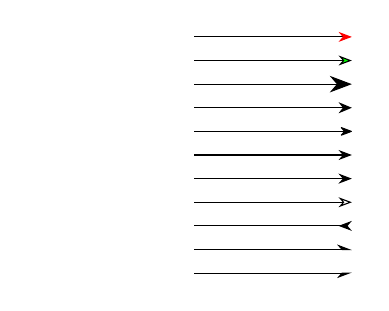
\begin{tikzpicture}
    \draw[-{Stealth[color=red]}] (0,0) -- (2,0);
    \draw[-{Stealth[fill=green]}] (0,-0.3) -- (2,-0.3);
    \draw[-{Stealth[length=8pt]}] (0,-0.6) -- (2,-0.6);
    \draw[-{Stealth[width=4pt]}] (0,-0.9) -- (2,-0.9);
    \draw[-{Stealth[round]}] (0,-1.2) -- (2,-1.2);
    \draw[-{Stealth[sharp]}] (0,-1.5) -- (2,-1.5);
    \draw[-{Stealth[line width=2pt,fill=none]}] (0,-1.8) -- (2,-1.8);
    \draw[-{Stealth[open]}] (0,-2.1) -- (2,-2.1);
    \draw[-{Stealth[reversed]}] (0,-2.4) -- (2,-2.4);
    \draw[-{Stealth[harpoon]}] (0,-2.7) -- (2,-2.7);
    \draw[-{Stealth[harpoon,swap]}] (0,-3.0) -- (2,-3.0);
    \node at (-2,-3){};
    \node at (2,0){};
\end{tikzpicture}
\end{document}
